\documentclass[10pt]{article}
\usepackage{icmlko}

\icmlmeta{IP 파운데이션 월드모델}{155}{손잡이인가 눈금인가}{손 축 다섯은 기획자가 돌리는 손잡이다. 백쉰 노트 만에 처음으로 ``돌리면 어떻게 되나''를 물었더니, 판을 제일 잘 맞히는 것들이 그 물음에는 답을 못 한다}

\begin{document}

\twocolumn[
\icmlheader

\begin{abstract}
손 축 다섯 --- 타깃 폭 · 장소 노출 · 입장 마찰 · 미디어 푸시 · 굿즈 규모 ---
은 전부 \textbf{기획자가 돌리는 손잡이}다. 그런데 백쉰 노트 동안 상관으로만
썼고 ``한 칸 올리면 어떻게 되나''를 물은 적이 없다. 월드모델과 랭커를
가르는 것이 그 물음이므로 물었다. 유보 레코드의 축 하나를 한 칸 올리고
예측이 어떻게 변하는지 잰다. \textbf{먼저 재는 자가 0을 강제하고
있었다} --- 현행 챔피언 F18 배깅은 예측이 순위 평균이라 모든 행을 같이
올리면 순위 합이 보존돼 평균 차가 \emph{정확히} 0이다. 36칸이 전부 0.000으로
나왔고, 효과가 없는 게 아니라 잴 수가 없는 것이었다. 눈금을 내는 F8 부스팅으로
바꿔 다시 쟀다. \textbf{사전 부호와 31/36 = 86\% 맞는다}(동전 50\%). 축별로
보면 타깃 폭 9/9 · 미디어 푸시 4/4 · 굿즈 규모 8/8로 셋은 손잡이처럼 굴고,
\textbf{입장 마찰은 4/8로 동전이고 장소 노출은 6/7이지만 평균 효과가
$+$0.068로 거의 없다} --- 게다가 하필 팝업에서 $-$0.058로 부호가 뒤집힌다.
그리고 진짜 시험을 했다. \textbf{모형이 함의하는 효과가 그 도메인의 자료와
맞는가.} 나머지 넷을 통제한 부분상관과 견주니 \textbf{순위상관이
$+$0.016이다 --- 관계가 없다.} 아이돌의 미디어 푸시는 모형이 $+$0.302인데
자료는 $-$0.214이고, 웹툰의 굿즈 규모는 모형 $+$0.185에 자료 $-$0.310이다.
정식화 넷을 다 대 봐도 같다(F8 $+$0.016 · F6 $+$0.010 · F9 $+$0.005 ·
F10 $-$0.119). \textbf{그리고 F10 도메인수축은 사전 부호를 5/36 = 14\% 밖에
못 맞힌다} --- 뒤집는 것이 규칙이다. 노트 147이 F10 을 판 2칸으로 올렸는데,
\textbf{판 2위가 손잡이로는 최악이다.} 결론은 하나다. 이 판의 정식화들은
\textbf{줄은 잘 세우고 손잡이는 못 돌린다.} 랭커이지 아직 월드모델이 아니다.
\end{abstract}
]

\begin{figure*}[t]
\centering
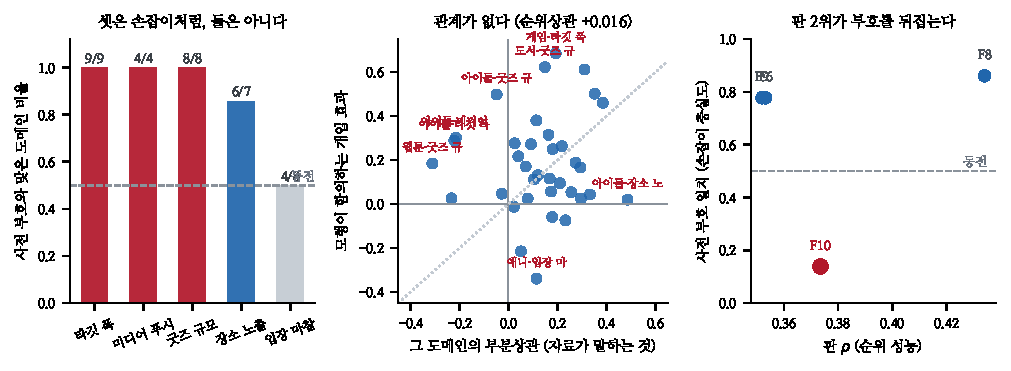
\includegraphics[width=\textwidth]{figs/lever.pdf}
\caption{왼쪽 --- 셋은 손잡이처럼, 둘은 아니다. 가운데 --- 모형이 함의하는
효과와 그 도메인의 자료 사이에 관계가 없다. 오른쪽 --- 판 2위가 부호를
뒤집는다.}
\end{figure*}

\section{먼저 재는 자가 0을 강제했다}

\claimx{\textbf{순위를 내는 정식화로는 개입을 못 잰다.} F18 배깅의 예측은
부스터 여덟의 \emph{순위 평균}이다. 모든 행의 축을 같이 올리면 순위 합이
보존되므로 평균 차가 정확히 0이 된다. 처음 표가 36칸 모두 $+$0.000이었고,
그것을 ``효과 없음''으로 읽을 뻔했다.}{노트 145에서 순위 평균을 고른 이유는
``눈금이 아니라 순위만 쓰는 판''이라서였다. 맞는 결정이었는데, 개입을 재는
순간 그 결정이 측정을 막는다. \textbf{좋은 채점 설계가 좋은 개입 설계는
아니다.}}

\section{셋은 손잡이처럼 군다}

\begin{table}[t]
\centering\tsize
\caption{축 한 칸($0\!\sim\!4$에서 $+$1)을 올렸을 때. F8 부스팅 · 씨앗 셋.}
\begin{tabular}{lrrr}
\toprule
& 사전 & 맞은 도메인 & 평균 효과 \\
\midrule
타깃 폭 & $+$ & \textbf{9/9} & $+$.284 \\
미디어 푸시 & $+$ & \textbf{4/4} & $+$.284 \\
굿즈 규모 & $+$ & \textbf{8/8} & $+$.330 \\
\midrule
장소 노출 & $+$ & 6/7 & $+$.068 \\
\textbf{입장 마찰} & $-$ & \textbf{4/8} & $-$.012 \\
\bottomrule
\end{tabular}
\end{table}

\claimx{\textbf{입장 마찰은 동전이다.} 8개 도메인 중 4개만 사전 부호와
맞고 평균 효과가 $-$0.012다. 세계애니 $-$0.214 · 애니 $-$0.339로 내려가는
곳이 있고 펀딩 $+$0.381 · 팝업 $+$0.095로 올라가는 곳이 있다.}{올라가는
쪽이 이상한 것이 아니다 --- 유료·사전예약을 거는 팝업은 원래 수요가 있는
팝업이다. 즉 선택이 개입을 덮는다. \textbf{그것이 바로 손잡이가 아니라는
뜻이다.}}

\claimx{\textbf{장소 노출은 팝업에서 부호가 뒤집힌다}($-$0.058). 노트 153이
잰 대로 팝업에서 장소 노출은 라벨과의 상관이 $+$0.441로 다섯 축 중 제일
높은데, 모형이 함의하는 개입 효과는 음수다.}{좋은 자리를 좋은 IP 가
가져간다 --- 교과서적인 교란이다. 상관이 제일 센 축이 손잡이로는 제일
못 미더울 수 있다.}

\section{진짜 시험 --- 자료와 맞는가}

사전 부호는 내 상식이지 자료가 아니다. 자료에 대 보려면 그 도메인에서
나머지 넷을 통제한 \textbf{부분상관}과 견줘야 한다.

\begin{table}[t]
\centering\tsize
\caption{어긋나는 자리. 모형 효과 대 그 도메인 부분상관.}
\begin{tabular}{llrr}
\toprule
& & 모형 & 자료 \\
\midrule
아이돌 & 미디어 푸시 & $+$.302 & \textbf{$-$.214} \\
웹툰 & 굿즈 규모 & $+$.185 & \textbf{$-$.310} \\
펀딩 & 입장 마찰 & $+$.381 & $+$.115 \\
팝업 & 장소 노출 & $-$.058 & $+$.179 \\
아이돌 & 굿즈 규모 & $+$.499 & $-$.048 \\
\bottomrule
\end{tabular}
\end{table}

\claimx{\textbf{순위상관이 $+$0.016이다 --- 관계가 없다.} 36칸에서 모형이
함의하는 개입 효과와 그 도메인의 부분상관 사이에 크기 관계가 없다. 부호만
69\% 맞고 그것도 동전보다 조금 나은 정도다.}{이 결과가 오히려 놀랍다.
처음에 걱정한 것은 반대였다 --- ``모형은 관측으로 적합했으니 관측을 재현할
뿐 아닌가.'' 재현조차 안 한다.}

\begin{table}[t]
\centering\tsize
\caption{정식화 넷. 전부 같다.}
\begin{tabular}{lrrr}
\toprule
& 사전 부호 & 자료와 상관 & 부호 일치 \\
\midrule
F8 부스팅 & \textbf{86\%} & $+$.016 & 69\% \\
F6 능형 & 78\% & $+$.010 & \textbf{83\%} \\
F9 순위우도 & 78\% & $+$.005 & \textbf{83\%} \\
\textbf{F10 도메인수축} & \textbf{14\%} & $-$.119 & 22\% \\
\bottomrule
\end{tabular}
\end{table}

\claimx{\textbf{F10 은 부호를 뒤집는 것이 규칙이다} --- 사전 부호를 5/36 =
14\% 밖에 못 맞힌다. 뒤집는 쪽이 86\%다. 노트 147이 짝 분해능으로 F10 을
판 2칸(선형 셋 위)으로 올렸는데, \textbf{그 2위가 손잡이로는 최악이다.}}{F10 은
도메인마다 수축을 다르게 주는 선형이다. 도메인 계수가 음수인 곳에서 수축이
그것을 증폭하면 이렇게 된다. 다만 14\%는 잡음이 아니라 체계적 역전이라
따로 파야 한다.}

\claimx{\textbf{판 순위와 손잡이 충실도가 어긋난다.} F8 이 사전 부호는 제일
잘 맞히고(86\%) 자료 부호는 제일 못 맞힌다(69\%). F6 · F9 는 반대다(78\% ·
83\%). 판 2위 F10 은 둘 다 최악이다.}{두 잣대가 다른 것을 재고 있다는
뜻이고, \textbf{지금 순위표는 손잡이 쪽을 아예 안 본다.}}

\section{그래서 어디쯤인가}

\claimx{\textbf{줄은 잘 세우고 손잡이는 못 돌린다.} 판 $\rho$ $+$0.45는
``두 IP 중 어느 쪽이 클까''를 64\% 맞힌다는 뜻이고 그것은 실재한다. 그런데
``이 IP 의 굿즈를 키우면 어떻게 되나''에는 어느 정식화도 자료와 맞는 답을
못 낸다(순위상관 $\le$ 0.02). \textbf{랭커이지 아직 월드모델이 아니다.}}{개입
효과의 참값을 우리는 모른다 --- 부분상관도 교란이 남는다. 그러니 여기서
말할 수 있는 것은 ``맞다''가 아니라 \textbf{``자료와도 안 맞는다''}까지다.
그것만으로도 충분히 나쁘다.}

\begin{table}[t]
\centering\tsize
\caption{남은 것.}
\begin{tabular}{ll}
\toprule
\textbf{F10 역전} & 14\%는 체계적이다 --- 수축의 어느 부분인가 \\
개입 판정치 & 순위표에 손잡이 충실도를 같이 싣는다 \\
반사실 자료 & 같은 IP 가 축만 달리해 두 번 나온 짝 12개뿐 \\
\bottomrule
\end{tabular}
\end{table}

둘째 줄이 규약이다. 이 판의 순위표는 판 $\rho$ 하나로 세우는데, 그것이
손잡이 쪽을 아예 안 보는 잣대임이 이 노트에서 드러났다. \textbf{실행마다
사전 부호 일치와 자료 부호 일치를 같이 적는다} --- 노트 144의 귀착, 노트
147의 짝 분해능에 이어 셋째 부기다.

\end{document}
